\documentclass[12pt]{report}
\usepackage{titling}
\usepackage{graphicx}
\usepackage[export]{adjustbox}

\title{Homework 2, Team C}
\author{ Kurt Blasdell (blas5260)
\and Elizabeth Hernandez (hern9899)
\and Jordan Lynn (lynn8983)
\and Brett Menzies (menz9375)
\and Michael Mueller (muel2767)
\and Ronald Rodriguez (rodr3849)
\and Lance Wells (well3112)
\and Zachary Yama (yama4272)
\and Jared Zook (jzook@uidaho.edu)
\and Morgan Holbart (holb5155)
}


\begin{document}
    \maketitle

\tableofcontents{}

\chapter{PlantUML Diagrams}
\begin{figure}
	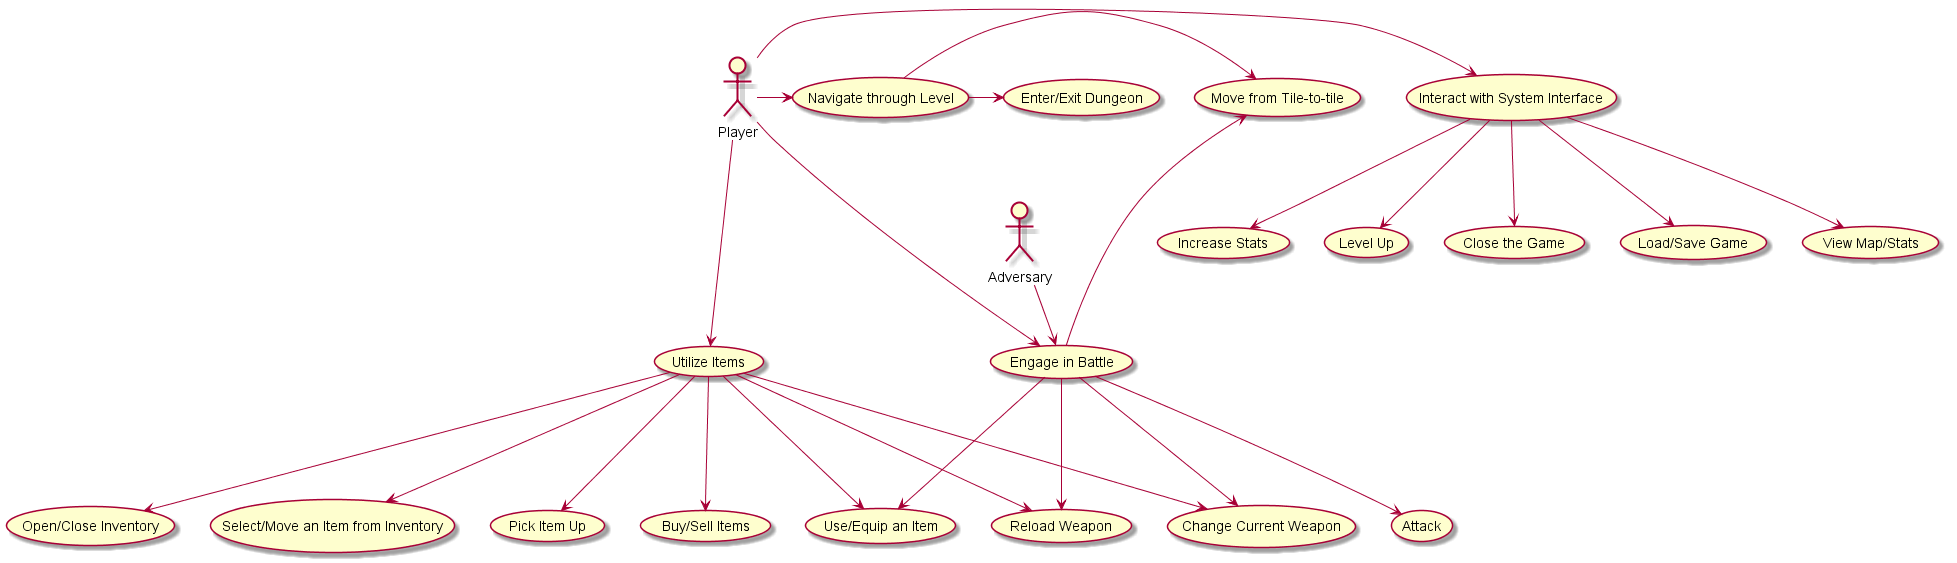
\includegraphics[scale=0.25,left]{uml-Jared_Zook.png}
	\caption{UML diagram - Jared Zook}
\end{figure}

\begin{figure}
	\centering
	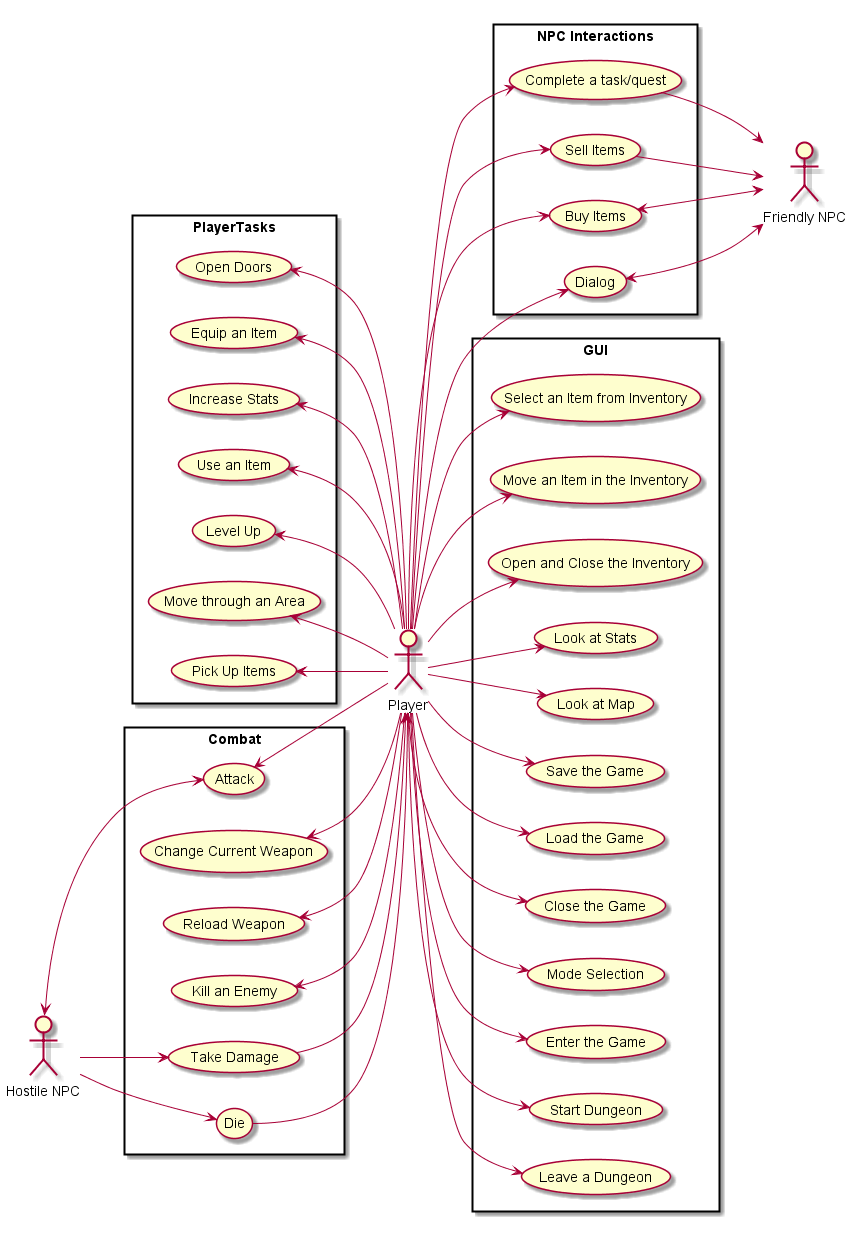
\includegraphics[scale=0.4,center]{uml-Lance_Wells.png}
	\caption{UML diagram - Lance Wells}
\end{figure}


\chapter{Use-Case Specifications}


\section{Kurt Blasdell}
\begin{subsection}{Open and Close the Inventory}
\textbf{Actor:} The Player. \\
\textbf{Goal:} Open the inventory, or close the inventory when finished. \\
\textbf{Summary:} The player opens up the inventory in order to view or use items, or the player closes the inventory when they are finished. \\
\textbf{Related Use-Cases:} Select an item from inventory; Move and item in the inventory \\
\textbf{Steps:}
\begin{enumerate}
	\item The player presses the ‘i’ key
	\item An inventory window will open, allowing the player to do things with items in the inventory
	\item Pressing the ‘i’ key again will close the inventory screen
\end{enumerate}
\textbf{Alternative:} The player may also click the Inventory window icon to open/close.
\end{subsection}

\begin{subsection}{Reload Weapon}
\textbf{Actor:} The Player. \\
\textbf{Goal:} The player’s weapon will be reloaded with ammo \\
\textbf{Precondition:} The player has a weapon equipped that takes some form of ammo. \\
\textbf{Precondition:} The player has the correct type of ammo for the weapon. \\
\textbf{Summary:} The player will fill their weapon with ammo that they may have. \\
\textbf{Steps:}
\begin{enumerate}
	\item Press the reload button
	\item Subtract the correct amount of ammo from the players ammo resources
	\item Add the amount from step two to the ammo in the player’s weapon
\end{enumerate}
\end{subsection}

\begin{subsection}{Look at Stats}
\textbf{Actor:} The Player. \\
\textbf{Goal:} Open the stats screen and close when the player if finished. \\
\textbf{Summary:} The player opens up the stats screen in order to view stats, or alter them, or the player closes the stats screen when they are finished. \\
\textbf{Related Use-Cases:} Increase Stats \\
\textbf{Steps:}
\begin{enumerate}
	\item The player presses the ‘c’ key
	\item The stats window is opened displaying current stats and stat points
	\item Pressing the ‘c’ key again will close the stats window
\end{enumerate}
\textbf{Alternative:} The player may also click the stats window icon to open/close.
\end{subsection}





\section{Elizabeth Hernandez}
\begin{subsection}{Move Avatar}
\textbf{Actor:} The Player \\
\textbf{Goal:} Change the position of the player's avatar \\
\textbf{Preconditions:} 
\begin{enumerate}
	\item The player is not viewing a selection screen
	\item The player's character is not suffering from an effect that prohibits movement
\end{enumerate}
\textbf{Summary:} The player directs their avatar to move into an adjacent space. \\
\textbf{Related Use-Cases:} Collect an Item, View the Map, Attacking an Enemy, Sustaining Damage, Dialogue, Buy an Item, Sell Items \\
\textbf{Steps:}
\begin{enumerate}
	\item The player moves their avatar into a space containing an item
	\item The player presses the selection key
	\item The item is removed from its space
	\item The item is added to the player's inventory
\end{enumerate}
\textbf{Alternatives:} 
\begin{enumerate}
	\item Step 1: The player faces their avatar at an adjacent space containing an item
	\item Step 4: The item is used immediately
\end{enumerate}
\end{subsection}

\begin{subsection}{Collect an Item}
\textbf{Actor:} The Player \\
\textbf{Goal:} Collect an item for use by player \\
\textbf{Preconditions:} \begin{enumerate}
	\item Avatar movement is allowed for the player
\end{enumerate}
\textbf{Summary:} The player collects an item from the immediate area. \\
\textbf{Related Use-Cases:} Move Avatar \\
\textbf{Steps:}
\begin{enumerate}
	\item The player moves their avatar into a space containing an item
	\item The player presses the selection key
	\item The item is removed from its space
	\item The item is added to the player's inventory
\end{enumerate}
\textbf{Alternatives:} 
\begin{enumerate}
	\item Step 1: The player faces their avatar at an adjacent space containing an item
	\item Step 4: The item is used immediately
\end{enumerate}
\end{subsection}

\begin{subsection}{View the Map}
\textbf{Actor:} The Player \\
\textbf{Goal:} Display where known objects are in relation to the player's avatar \\
\textbf{Preconditions:} 
\begin{enumerate}
	\item Avatar movement is allowed for the player
\end{enumerate}
\textbf{Summary:} The player views a large-scale map of their current area. \\
\textbf{Related Use-Cases:} Move Avatar, Enter a Dungeon, Leave a Dungeon \\
\textbf{Steps:}
\begin{enumerate}
	\item The player presses the map key
	\item The player's standard view of the area is replaced by a map of the area
	\item The player moves their avatar
	\item The player presses either the escape key or map key
	\item The player's view of the area is returned to its standard formatr
\end{enumerate}
\textbf{Alternatives:} 
\begin{enumerate}
	\item Step 3: The player chooses to enter or leave a dungeon
	\item Step 3: The player proceeds directly to Step 4
\end{enumerate}
\end{subsection}




\section{Jordan Lynn}
    \subsection{Sell Items}
    
    \subsubsection{Actors}
    \begin{itemize}
        \item Player
        \item Shopkeeper
        \item Wharehouse Manager
        \item Second Player
    \end{itemize}

    \subsubsection{Preconditions}
    \begin{itemize}
        \item Player or Players must be in close proximity of each other.
        \item Two trading parties looking to purchase must have enough money for exchange.
    \end{itemize}

    \subsubsection{Summary}
    Player will exchange item for currency with another player or shopkeeper.

    \subsubsection{Steps}
    \begin{enumerate}
        \item Player comes in close proximity of second party to trade with.
        \item Player intiates trading menu.
        \item Player selects item to sell from inventory.
        \item Player confirms sell.
            \begin{enumerate}
                \item If second party is another player that player too confirms sell.
            \end{enumerate}
        \item Currency is taken from the second party and given to the player, as well the item is taken from the player's inventory.
    \end{enumerate}

    \subsection{Close the Game}
        \subsubsection{Actors}
        \begin{itemize}
            \item Player
        \end{itemize}

        \subsubsection{Preconditions}
        \begin{itemize}
            \item Acess to menu
        \end{itemize}

        \subsubsection{Summary}
        The player ends the game by closing it through the in game menu.

        \subsubsection{Steps}
        \begin{itemize}
            \item Player opens in game menu and selects "End Game".
            \item Player will comfirm exit of game.
            \item Game will auto-save and close.
        \end{itemize}






\section{Brett Menzies}

\begin{subsection}{Equip an Item}
\textbf{Actors:} Player \\
\textbf{Preconditions:} Play has an equitable item, and the necessary skill to use the item \\
\textbf{Summary:} The Player equips an item, changing their stats appropriately \\
\textbf{Terminates:} When item is equipped or returned to inventory \\
\textbf{Related use cases:} Select an Item from Inventory \\
\textbf{Steps:}

\begin{enumerate}
	\item The user Selects an Item from Inventory
	\item The user clicks on an equipment slot on their equipment display.
	\item The system checks if the active item is equitable in that location and the user has the necessary skill.
	\begin{itemize}
		\item If valid: system equips the active item to character and recalculates player stats,
			transporting previously equipped items to inventory if necessary.
		\item If invalid: system prints message in dialog box explaining what conditions failed.
	\end{itemize}
	\item Alternative: The user right-clicks anywhere, deactivating and returning the item to its previous location.
\end{enumerate}
\end{subsection}

\begin{subsection}{Use an Item}
\textbf{Actors:} Player \\
\textbf{Preconditions:} Player has usable item in inventory, valid target, and necessary skill \\
\textbf{Summary:} The Player uses his/her skill to use an item on a target \\
\textbf{Terminates:} After item is consumed or returned to inventory \\
\textbf{Related use cases:} Select an Item from Inventory \\
\textbf{Steps:}

\begin{enumerate}
	\item The user Selects an Item from Inventory
	\item The user clicks on a target map tile.
	\item The system checks if the target is valid and the user has the necessary skill to use the active item.
	\begin{itemize}
		\item If valid: system applies items effects to target; item is consumed.
		\item If invalid:  system prints message in dialog box explaining what conditions failed.
	\end{itemize}
	\item Alternative: The user right-clicks anywhere, deactivating and returning the item to its previous location.
\end{enumerate}

\end{subsection}





\section{Michael Mueller}
\begin{subsection}{Killing an Enemy}
\textbf{Actors:} Player,Enemy \\
\textbf{Goal:} Remove an eliminated enemy \\
\textbf{Preconditions:}
\begin{enumerate}
       \item Player is able to attack enemy
       \item Enemy has low enough armor to be fatally wounded this attack
\end{enumerate}
\textbf{Summary:} The player attacks an enemy, dealing a lethal blow. \\
\textbf{Related Use-Cases:} Attack, Leveling up, dialog \\
\textbf{Steps:}
\begin{enumerate}
	\item Player get close enough to attack the enemy
	\item Player attacks, slaying the enemy
	\item Enemy rewards the player
\end{enumerate}
\end{subsection}
\begin{subsection}{Die}
\textbf{Actors:} Player \\
\textbf{Goal:} Lose the game \\
\textbf{Preconditions:}
\begin{enumerate}
       \item Player has just recieved a fatal amount of damage
\end{enumerate}
\textbf{Summary:} The player was dealt a lethal blow dislaying loss dialog and choice to restart. \\
\textbf{Related Use-Cases:} Attack, Dialog, close the game \\
\textbf{Steps:}
\begin{enumerate}
	\item Player takes a form of lethal damage
	\item The game displays a possible death animation
	\item Game Over dialog
	\item Pop up menu of choices appears
	\item Player choices what to do
\end{enumerate}
\end{subsection}




\section{Ronnie Rodriguez}
\begin{subsection}{Increase Stats}
\textbf{Actor:} The Player. \\
\textbf{Goal:} Recieve stat boosts after obtaining sufficient experience points. \\
\textbf{Precondition:} The player has obtained sufficient experience points to increase in level, thus enabling a stat boost. \\
\textbf{Summary:} The player chooses which stats they would like to apply a permanent boost to after increasing in level.  \\
\textbf{Related Use-Cases:} Level Up \\
\textbf{Steps:}
\begin{enumerate}
	\item Player opens menu via input.
	\item Player navigates to 'Player Stats' section of menu.
	\item Player has 5 points they can distribute among different stats like Def, Atk, Mag, etc.
	\item Player navigates to stats using controller input and applies points accordingly.
	\item Player selects 'confirm' button in stats menu.
	\item ''Confirm point allocation?" prompt displays along with yes and no options.
	\item If no is selected, prompt goes away and player can continue to allocate points as desired.
	\item If yes is selected, prompt closes and permanent stat boosts are initiated in accordance with point allocation.
\end{enumerate}
\textbf{Alternative:} The Player has not increased in level, and therefore has no points to increase stats with.
\end{subsection}

\begin{subsection}{Level Up}
\textbf{Actor:} The Player. \\
\textbf{Goal:} Kill enough enemies and/or complete enough tasks to gain enough experience points to increase in level. \\
\textbf{Precondition:} The player is killing enemies and completing quests, which grants them experience points. \\
\textbf{Summary:} The player obtains enough experience points to increase in level, which grants them points to permanently increase their stats. \\
\textbf{Related Use-Cases:} Increase Stats \\
\textbf{Steps:}
\begin{enumerate}
	\item Player has not yet obtained the amount of experience points required to level up.
	\item Player kills enemy or completes quest that puts them at the required amount of experience points to level up.
	\item ''Level Up!" prompt displays with accompanying victory sound. Gameplay is not interrupted.
	\item Player initiates 'Increase Stats' procedure (see above).
\end{enumerate}
\textbf{Alternative:} The player has not obtained enough experience points to increase in level.
\end{subsection}

\begin{subsection}{Move Item in Inventory}
\textbf{Actor:} The Player. \\
\textbf{Goal:} Rearrange items within the inventory to allow for better organization and faster access \\
\textbf{Precondition:} The player has item(s), and they would like to rearrange those items within the inventory \\
\textbf{Summary:} The player chooses an item and then the spot they would like to move that item to within the inventory \\
\textbf{Related Use-Cases:} Equip an Item, Use an Item \\
\textbf{Steps:}
\begin{enumerate}
	\item Player opens menu via input.
	\item Player navigates to 'Inventory' section of menu.
	\item Player chooses 'Rearrange' option in 'Inventory' section.
	\item Player chooses item to move via input.
	\item Item chosen is highlighted.
	\item Player navigates to spot in inventory they would like to move item to.
	\item Player selects desired spot via input.
	\item If spot selected is empty, highlighted item is moved to this spot and item's previous spot becomes empty.
	\item If spot selected is not empty, highlighted item is moved to this spot and item that was previously occupying the selected spot is moved to original item's spot.
\end{enumerate}
\textbf{Alternative:} The Player has no items, and therefore nothing to rearrange.
\end{subsection}




\section{Lance Wells}

\begin{subsection}{Buy an Item}
\textbf{Actor:} The Player. \\
\textbf{Goal:} Purchase an item and have it placed in the inventory. \\
\textbf{Precondition:} The player has access to a merchant that is able to sell items \\
\textbf{Summary:} The player loses some currency in exchange for an item placed in their inventory \\
\textbf{Related Use-Cases:} Sell an item; Dialog \\
\textbf{Steps:}
\begin{enumerate}
	\item Be close enough to the merchant to be able to communicate.
	\item Begin dialog with the merchant.
	\item Select a ''buy" option.
	\item Indicate a desired item from the display.
	\item Merchant detracts the specified amount of money from the player.
	\item Receive an item in inventory.
\end{enumerate}
\textbf{Alternative:} The Player does not have enough money and receives a message indicating such.
\end{subsection}

\begin{subsection}{Enter a Dungeon}
\textbf{Actor:} The Player. \\
\textbf{Goal:} Enter a dungeon from some sort of menu option. \\
\textbf{Precondition:} The player has access to the option to enter a dungeon and is not currently in a dungeon \\
\textbf{Summary:} The player begins to play in a dungeon after a menu option \\
\textbf{Related Use-Cases:} Leave a Dungeon \\
\textbf{Steps:}
\begin{enumerate}
	\item Select an ''Enter Dungeon" button.
	\item Select a ''Confirm" button.
	\item Be moved into a dungeon environment.
\end{enumerate}
\end{subsection}

\begin{subsection}{Leave a Dungeon}
\textbf{Actor:} The Player. \\
\textbf{Goal:} Leave a dungeon from some sort of menu option. \\
\textbf{Precondition:} The player has access to the option to leave a dungeon and is currently in a dungeon \\
\textbf{Summary:} The player leaves a dungeon and is moved to some menu or lobby \\
\textbf{Related Use-Cases:} Enter a Dungeon \\
\textbf{Steps:}
\begin{enumerate}
	\item Request a ''Leave this dungeon" menu through some button press.
	\item Select a ''Confirm" button.
	\item Be moved into a specified menu environment.
\end{enumerate}
\end{subsection}

\begin{subsection}{Dialog}
\textbf{Actors:} The Player, Friendly NPC \\
\textbf{Goal:} Converse with an NPC to a desired plot point. \\
\textbf{Precondition:} The player has access to a conversable NPC. \\
\textbf{Summary:} The player navigates a conversation via contextual button presses. \\
\textbf{Related Use-Cases:} Buy an Item, Sell an Item. \\
\textbf{Steps:}
\begin{enumerate}
	\item The player indicates a request to communicate with a nearby NPC via a button press.
	\item A box with ''greeting" dialog is displayed.
	\item The player must then press buttons with according textual decisions to communicate.
	\item The player closes the conversation with a ''Goodbye" textual decision button.
\end{enumerate}
\end{subsection}

\begin{subsection}{Multiplayer Selection}
\textbf{Actors:} The Player \\
\textbf{Goal:} Select a menu option to begin either single-player or multi-player mode. \\
\textbf{Precondition:} The player must be at a menu with the option to begin playing. \\
\textbf{Summary:} The player picks the 'multi-player' option from a menu and is sent to host a session or join a section. Multiplayer will work through a system where each player is playing in real time with eachother. Situations like attacking will be pseudo-turn based by having a cool down on each attack. This will allow our system to seem turn based when really it is real time.
\textbf{Steps:}
\begin{enumerate}
	\item The player selects 'multi-player'.
	\item The player is then directed into a menu which prompts the user to either host or join a session.
	\item The player picks 'host'.
	\item The player is then sent into a game with the option for users to join at-will.
\end{enumerate}
\textbf{Alternative:}
\begin{enumerate}
	\item (Step 1): The player picks 'single-player' and is sent into the game without the option for other players to join.
	\item (Step 4): The player picks 'join' and is sent to a menu which prompts the user for an ip address which then connects them with a host.
\end{enumerate}
\end{clearsubsection}

\begin{subsection}{Complete a task/quest}
\textbf{Actors:} The Player, Friendly NPC \\
\textbf{Goal:} The player successfully completes a quest \\
\textbf{Precondition:} The player must have completed all tasks for a quest. \\
\textbf{Summary:} The player opens a quest log and completes a quest through a series of button presses. \\
\textbf{Steps:}
\begin{enumerate}
	\item The player opens a 'quest log'.
	\item The player indicates which quest that they would like to attempt to complete via some button press.
	\item The player indicates that they would like to complete that quest via some button press.
	\item The player completes a quest and all according rewards are split into  respective inventories.
	\item The quest is now indicated as being complete for the hosting player.
\end{enumerate}
\textbf{Alternative:} The player does not have all objectives complete and cannot choose to complete the quest.
\end{subsection}

\begin{subsection}{Start the game}
\textbf{Actors:} The Player \\
\textbf{Goal:} The player successfully starts the game. \\
\textbf{Precondition:} The player must not have the game already started. \\
\textbf{Summary:} The player starts the game through the java virtual machine and is directed to a main menu. \\
\textbf{Steps:}
\begin{enumerate}
	\item The player chooses to run the game through the java virtual machine.
	\item The game begins, transitioning to a main menu.
\end{enumerate}
\end{subsection}

\begin{subsection}{Open doors}
\textbf{Actors:} The Player \\
\textbf{Goal:} The player successfully opens a door. \\
\textbf{Precondition:} The player must be within operable range of a door. \\
\textbf{Summary:} The player opens a door after checking for keys and codes. \\
\textbf{Steps:}
\begin{enumerate}
	\item The player indicates that they would like to open a door through some button press.
	\item The door is then checked to see if it requires any sort of keys/codes or if it is locked.
	\item If the door is locked, the player is then prompted for a key or a code.
	\item If the door requires a key, an appropriate key is then removed from the player's inventory.
	\item The door is unlocked.
	\item The door is opened.
\end{enumerate}
\textbf{Alternative:}
\begin{enumerate}
	\item (Step 3): If the door requires no key, or is not locked, the door opens without further prompts.
	\item (Step 4): If the door requires no key, but requires a code, the player is then prompted for a code which is entered via a keypad.
	\item (Step 5): If the player does not have the appropriate key, the player is then informed as such and the door remains locked.
\end{enumerate}
\end{subsection}

\begin{subsection}{Change Current Weapon}
\textbf{Actors:} The Player \\
\textbf{Goal:} The player successfully changes their currently equipped weapon. \\
\textbf{Precondition:} The player must have two or more weapons ready to change. \\
\textbf{Summary:} -------------------------------- \\
\textbf{Steps:}
\begin{enumerate}
	\item The player indicates that they would like to change weapons through some button press (e.g. 1,2,3,etc.)
	\item The system then checks if the player has a weapon in the desired slot (e.g. 1,2,3,etc.)
	\item If the player has a weapon in that selected slot, the player's active weapon is then changed to that weapon, leaving the old weapon in-tact.
\end{enumerate}
\textbf{Alternative:}
\begin{enumerate}
	\item (Step 3): If the player does not have an equipped weapon in that slot, the player then switches to an empty hand.
\end{enumerate}
\end{subsection}





\section{Zachary Yama}

\begin{subsection}{Attacking}
\textbf{Actor:} The Player
\textbf{Goal:} Deal damage to an enemy or object and destroy it.
\textbf{Preconditions:}
\begin{enumerate}
	\item The player is allowed and has the ability to attack.
	\item The player has a vaild weapon to attack with.
	\item The player has enough ammunition or duribility to attack.
\end{enumerate}
\textbf{Summary:} The player attacks and entity, dealing some damage.
\textbf{Related Use-Cases:} Kill an Enemy, Reload Weapon
\textbf{Steps:}
\begin{enumerate}
	\item The player uses the attack action.
	\item A valid hitbox collision is checked for.
	\item Ammunition and/or duribility are reduced.
	\item Damage is calculated and applied to any hit entities.
	\item Visual elements are instantiated.
\end{enumerate}
\end{subsection}

\begin{subsection}{Reloading Weapon}
\textbf{Actor:} The Player
\textbf{Goal:} Replenish weapon ammunition.
\textbf{Preconditions:}
\begin{enumerate}
	\item The player is allowed and has the ability to reload.
	\item The player has a vaild weapon to reload with.
	\item The player has enough ammunition to reload.
\end{enumerate}
\textbf{Summary:} The player decides to replenish their weapon(s) ammunition.
\textbf{Related Use-Cases:} Attack
\textbf{Steps:}
\begin{enumerate}
	\item The player uses the reload action.
	\item Inventory ammunition is reduced by the amount held in the weapon(s).
	\item Weapons ammunition is replenished.
	\item Visual elements are instantiated.
	\item Ignoring input for some time or other side effects are applied.
\end{enumerate}
\end{subsection}

\begin{subsection}{Take Damage}
\textbf{Actor:} The Player, NPC, Enemy, Wall, Entity
\textbf{Goal:} Reduce an entities health.
\textbf{Preconditions:}
\begin{enumerate}
	\item The entity is damageable.
	\item The entity is not already destroyed.
	\item The entity has collided with a damaging component.
\end{enumerate}
\textbf{Summary:} An entity has been damaged and health is reduced accordingly.
\textbf{Related Use-Cases:} Attack
\textbf{Steps:}
\begin{enumerate}
	\item Calculate and apply damage received.
	\item Reduce armor duribility.
	\item Apply side effects.
	\item Visual elements are instantiated.
\end{enumerate}
\end{subsection}





\section{Jared Zook}

\begin{subsection}{Save the Game}
\textbf{Actor:} A single player. \\
\textbf{Goal:} Avoid starting the game over by saving progress. \\
\textbf{Precondition:} The player is not engaged in battle. \\
\textbf{Summary:} Save points are placed in specified locations found just prior to boss battles. They are represented as items. The player engages the save, chooses a name for their file, and saves the game.  \\
\textbf{Related Use-Cases:} Pick Up Items, Use an Item \\
\textbf{Steps:}
\begin{enumerate}
   \item Player picks up the save item.
   \item Player selects a slot to save the game from menu.
   \item Player enters a name for the saved location.
   \item Player selects ''Save" button.
\end{enumerate}
\textbf{Alternatives:} The player exits the menu wthout saving.
\textbf{Postcondition:} Player returns to normal gameplay. Player's location, stats, and inventory are saved for later use.
\end{subsection}

\begin{subsection}{Load the Game}
\textbf{Actor:} A single player. \\
\textbf{Goal:} Retain the progress made from playing previously. \\
\textbf{Precondition:} The player previously saved at least one game. \\
\textbf{Summary:} The player can resume play at last saved location with inventory and stats intact.  \\
\textbf{Related Use-Cases:} Save Game, Select Item from Inventory \\
\textbf{Steps:}
\begin{enumerate}
   \item Player selects ''Load Game" menu from start menu.
   \item Player selects the slot to load.
\end{enumerate}
\textbf{Alternative:} The player begins a new game.
\textbf{Postcondition:} The player's chosen previous location, stats, and inventory are restored.
\end{subsection}

\begin{subsection}{Select an Item}
\textbf{Actor:} A Single Player. \\
\textbf{Goal:} To enable the ability for the player to use an item. \\
\textbf{Precondition:} The player is not viewing any other menu. \\
\textbf{Summary:} The player selects an item from inventory, such as a weapon, and is then free to equip it. \\
\textbf{Related Use-Cases:} Equip an Item \\
\textbf{Steps:}
\begin{enumerate}
   \item Player enters inventory.
   \item Player scrolls down to desired item.
   \item Player chooses ''Select".
\end{enumerate}
\end{subsection}


\section{Morgan Holbart}
\begin{subsection}{Enter the Game}
\textbf{Actor:} A Player. \\
\textbf{Goal:} Start the game from the menu \\
\textbf{Preconditions:}
\begin{enumerate}
	\item The player is currently in the starting menu
\end{enumerate}
\textbf{Summary:} The player attempts to start the game \\
\textbf{Related Use-Cases:} Load Game \\
\textbf{Steps:}
\begin{enumerate}
	\item The player selects the start button
	\item The player presses the input to activate the start button
\end{enumerate}
\end{subsection}
\begin{subsection}{Open Doors w/ Regard to Keys}
\textbf{Actor:} A Player. \\
\textbf{Goal:} Open a door adjacent to the player \\
\textbf{Preconditions:}
\begin{enumerate}
	\item The player is standing adjacent to the door
	\item The player has any key required to open the door
	\item The player is not currently in combat
\end{enumerate}
\textbf{Summary:} The player stands next to a door, faces it, presses the use action, and the door opens if he holds the key \\
\textbf{Related Use-Cases:} Move Through an Area, Interact, Move Avatar \\
\textbf{Steps:}
\begin{enumerate}
	\item The player moves adjacent to a door
	\item The player faces the door
	\item The player interacts with the door
\end{enumerate}
\end{subsection}
\begin{subsection}{Craft Item}
\textbf{Actor:} A Player. \\
\textbf{Goal:} Craft an item. \\
\textbf{Preconditions:}
\begin{enumerate}
	\item The player has selected X components to craft together from the crafting menu
	\item The player has the selected components in his inventory
	\item The components selected to craft together will compile into a valid recipe
	\item The player has an inventory slot available to put the crafted item in
\end{enumerate}
\textbf{Summary:} The player selects components to craft, if he has the components and an inventory space, and it makes a valid recipe, it will craft the item. \\
\textbf{Related Use-Cases:} Open Crafting Screen \\
\textbf{Steps:}
\begin{enumerate}
	\item The player opens the crafting screen
	\item The player selects a number of components
	\item The player presses the craft button
\end{enumerate}
\end{subsection}

\end{document}
